% Contributors: Alexandre Lamy, Trung Vu
\section{The watershed algorithm}
  The watershed algorithm is another density based clustering method, often used in image classification.
  The algorithm has two steps. First it estimates the density of the distribution over the space (i.e. 
  it estimates the probability density function (PDF) of the distribution from which it assumes that the data points
  have been drawn). We will see exactly how this can be done in later sections. 
  
  Then the algorithm will ``flip'' the estimated PDF and start ``filling it with water''. Regions where water from different
  ``wells'' touch for the first time will become cluster boundaries.
  
  \begin{figure}[h]
  \centering
  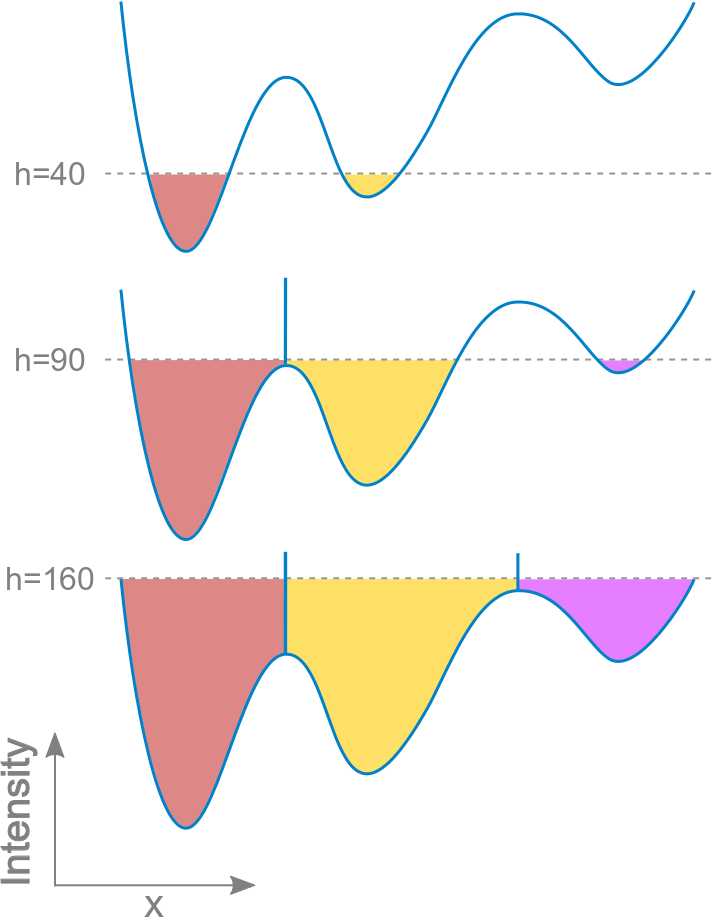
\includegraphics[width=.7\linewidth]{chapter_2/files/Watershed-flooding-graph.png}
  \caption{Watershed 1D visualization }
  \end{figure}
  
  \begin{figure}[h]
  \centering
  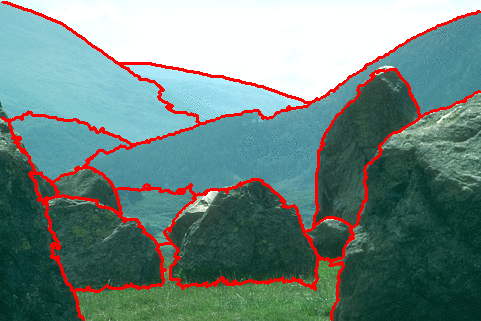
\includegraphics[width=.7\linewidth]{chapter_2/files/PW_overlay.png}
  \caption{2D images clustering using watershed}
  \end{figure}
